\section{Perspectiva histórica}

\begin{frame}[t]{Tecnología}

\mode<presentation>{\vspace{-1em}}
\begin{columns}[T]

\column{.45\textwidth}
\textgood{ASCI Red Computer}: \textemph{1.3 TFLOPS}\\
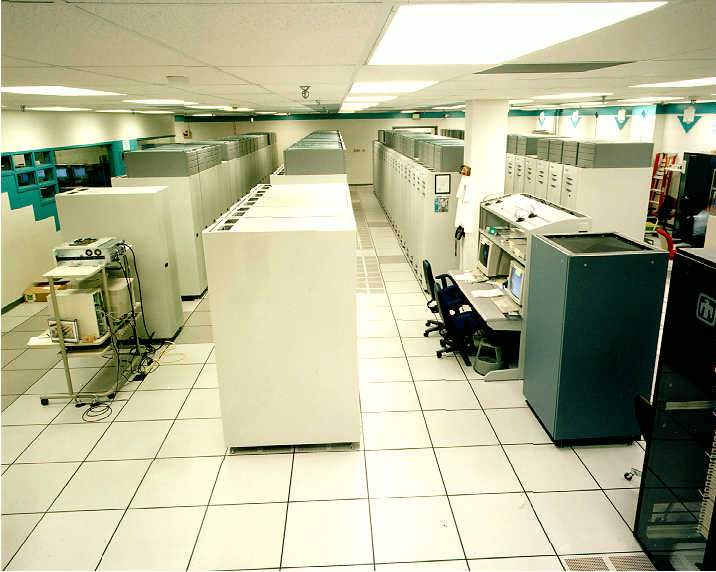
\includegraphics[height=.6\textheight]{images/asci-red.jpg}\\
\begin{tiny}
By Sandia National Laboratories, Public Domain\\
\url{https://commons.wikimedia.org/w/index.php?curid=28171282}\\
\end{tiny}

\textmark{1997}\\

\pause

\column{.55\textwidth}
\textgood{Samsung S22}: \textemph{1.2 -- 2.2 TFLOPS}\\
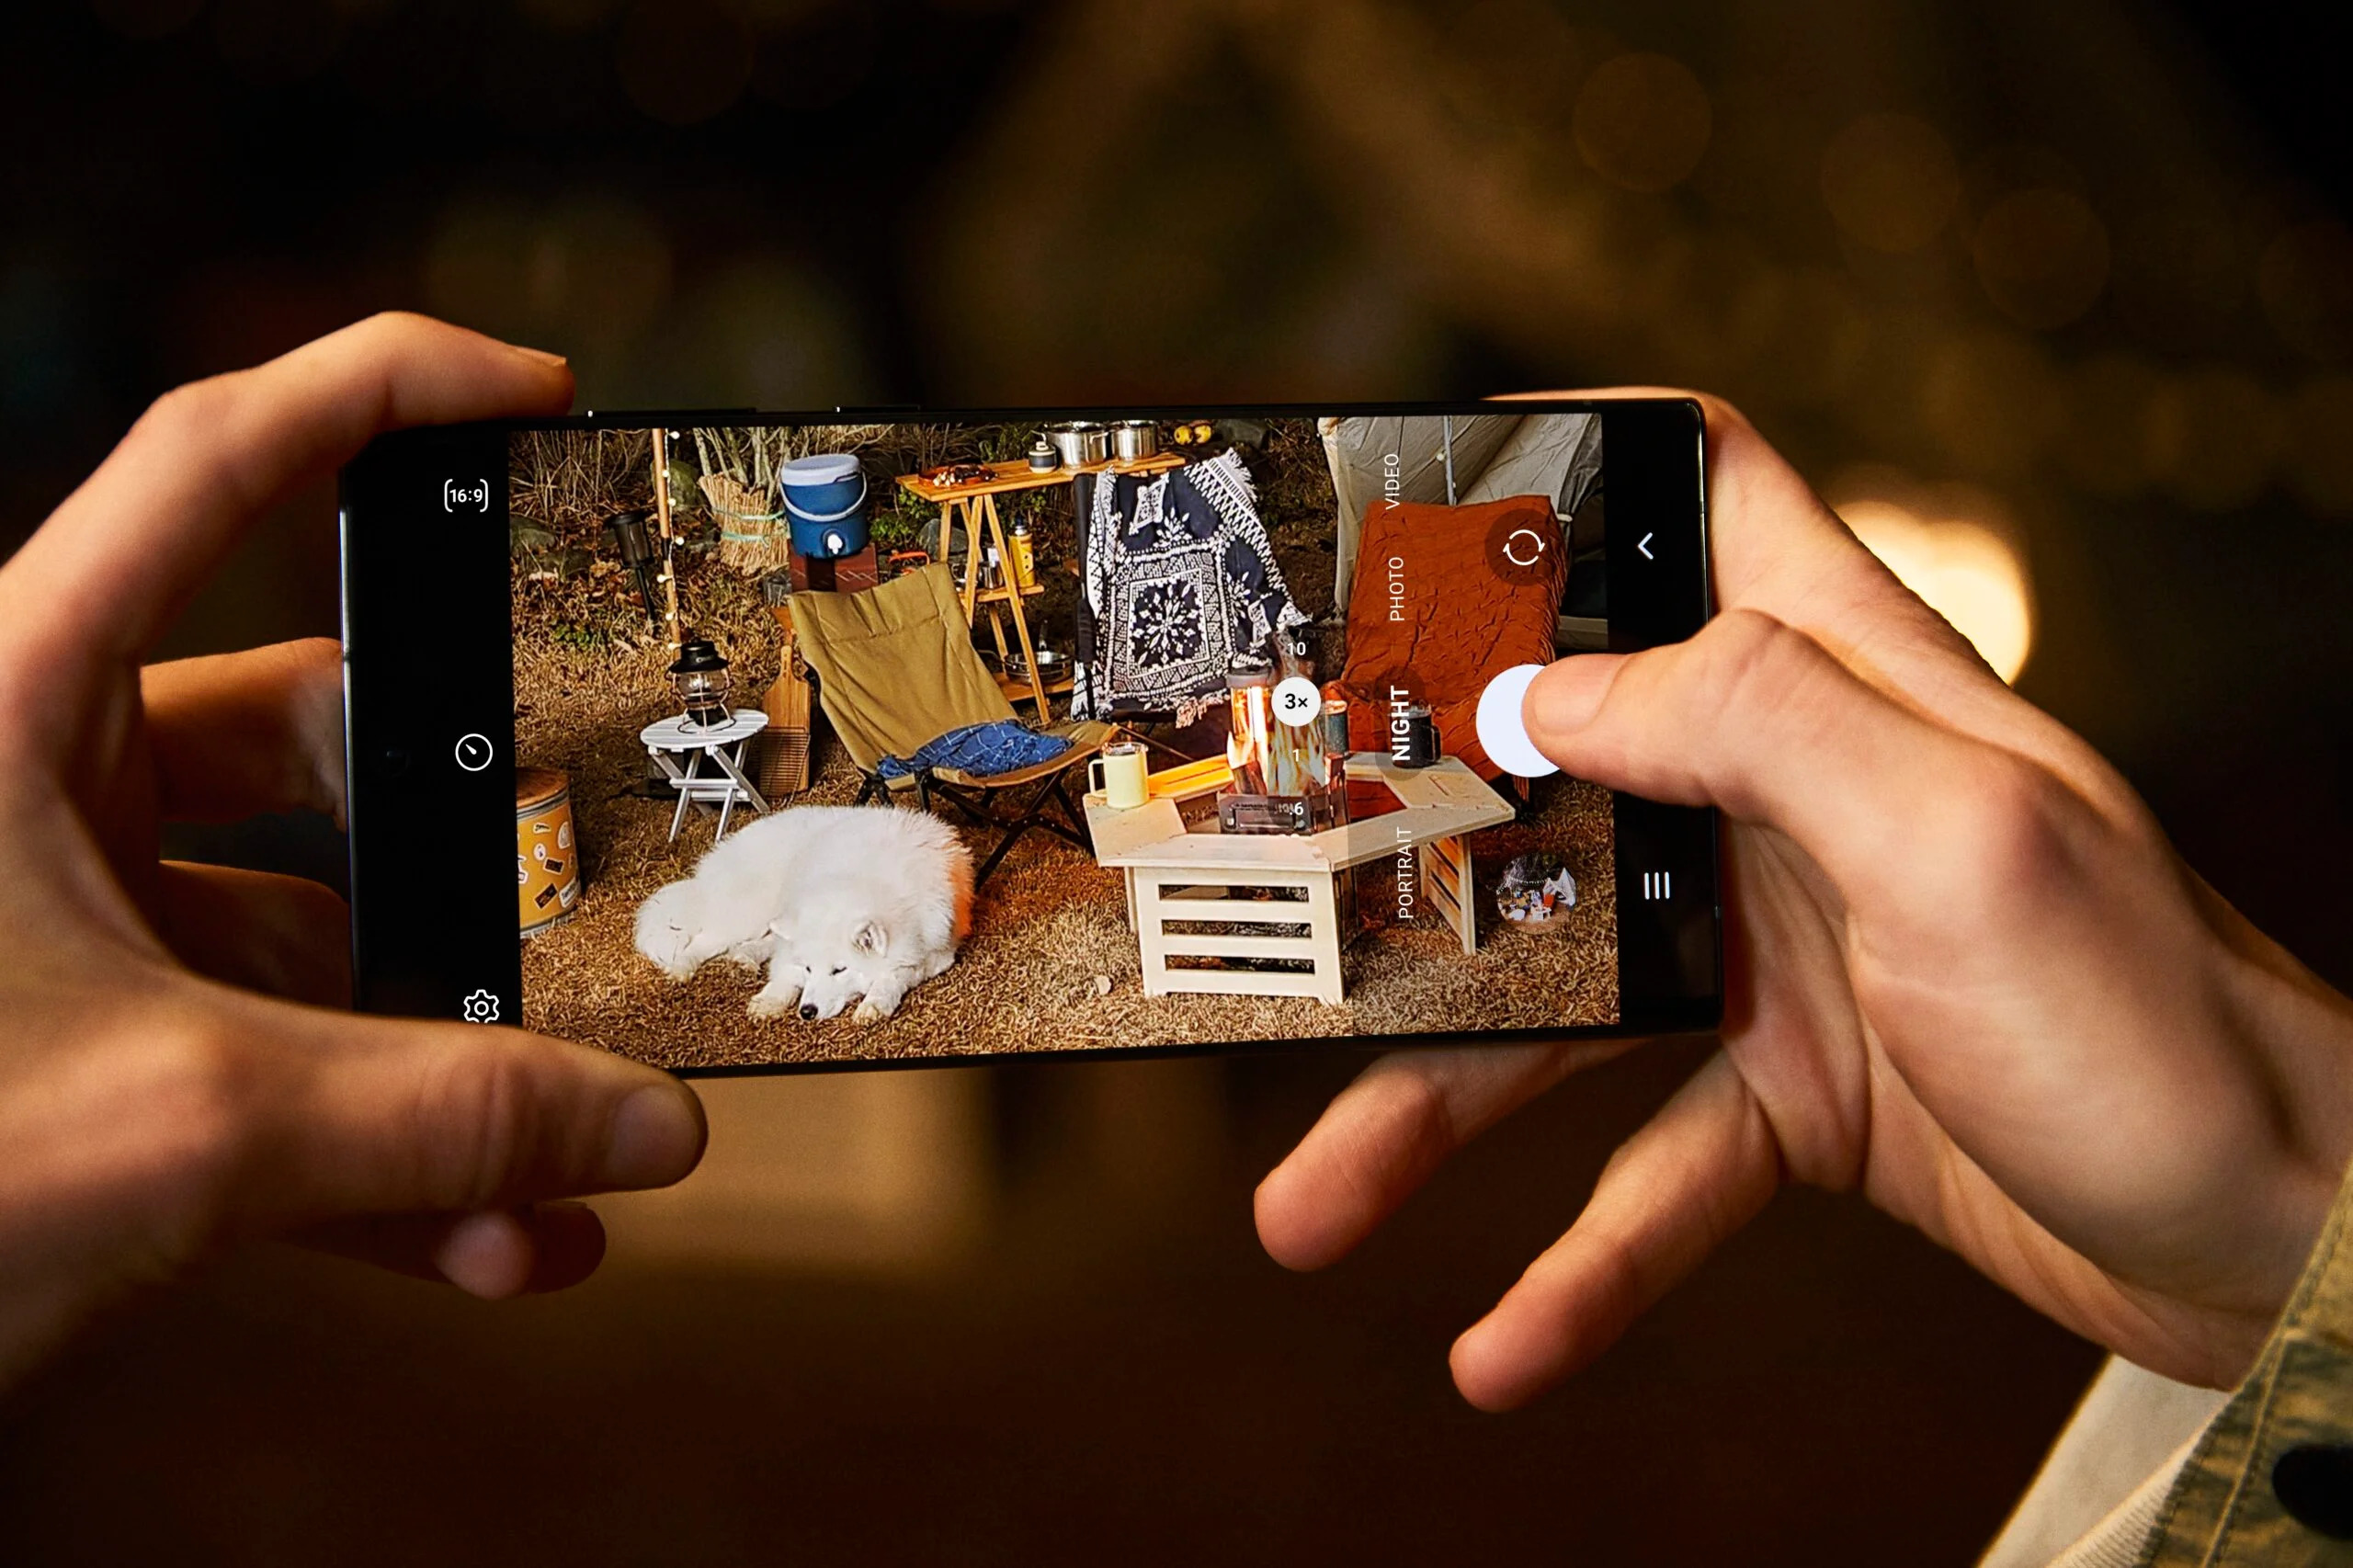
\includegraphics[height=.6\textheight]{images/samsung-s22.jpg}\\
\begin{tiny}
By Trusted Reviews, Creative Commons BY-NC-ND 4.0\\
{\begin{spacing}{1.0}
\url{https://www.trustedreviews.com/versus/samsung-galaxy-s22-ultra-vs-samsung-galaxy-s22-plus-vs-samsung-galaxy-s22-4207904}
\end{spacing}}
\end{tiny}

\textmark{2022}\\

\end{columns}

\end{frame}


\begin{frame}[t]{Primera revolución: El microprocesador}
\begin{itemize}
  \item La revolución del microprocesador.
    \begin{itemize}
      \item Generada a partir de un único cambio.
      \item Suficientes transistores (25,000) en un único chip para un procesador de 16 bits.
      \item \textgood{Ventajas}:
        \begin{itemize}
          \item \textmark{Más rápido}: Menos salidas del chip.
          \item \textmark{Más barato}: Todo en un chip.
        \end{itemize}
    \end{itemize}
  \item Nuevos segmentos de mercado generados por la innovación.
    \begin{itemize}
      \item Computadores de escritorio, CD/DVD, portátiles, consolas de videojuego,
            decodificadores TV, cámaras digitales, MP3, GPS, \ldots
    \end{itemize}
  \item Impacto en mercados existentes:
    \begin{itemize}
      \item Supercomputadores, \emph{mainframes}, \ldots
    \end{itemize}
\end{itemize}
\end{frame}

\begin{frame}[t]{Primer microprocesador}
\begin{columns}[T]
  \begin{column}{.7\textwidth}
    \begin{itemize}
      \item Intel 4004 (1971).
        \begin{itemize}
          \item \textmark{Dominio de aplicación}: Calculadoras.
          \item \textmark{Tecnología}: 10,000 nm.
          \mode<presentation>{\vfill}
          \item \textgood{Datos}:
            \begin{itemize}
              \item 2300 transistores.
              \item 13 mm2.
              \item 108 KHz.
              \item 12 Voltios.
            \end{itemize}
          \mode<presentation>{\vfill}
          \item \textgood{Características}:
            \begin{itemize}
              \item Datos de 4 bits.
              \item Camino de datos en un ciclo.
            \end{itemize}
      \end{itemize}
    \end{itemize}
  \end{column}
  \begin{column}{.3\textwidth}
    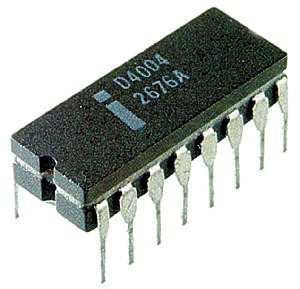
\includegraphics[width=.5\textwidth]{images/intel-4004.jpg}\\
    \begin{tiny}
      \emph{Intel 4004}, foto de Rostislav Lisovy\\
    \end{tiny}
    \vspace{1em}
    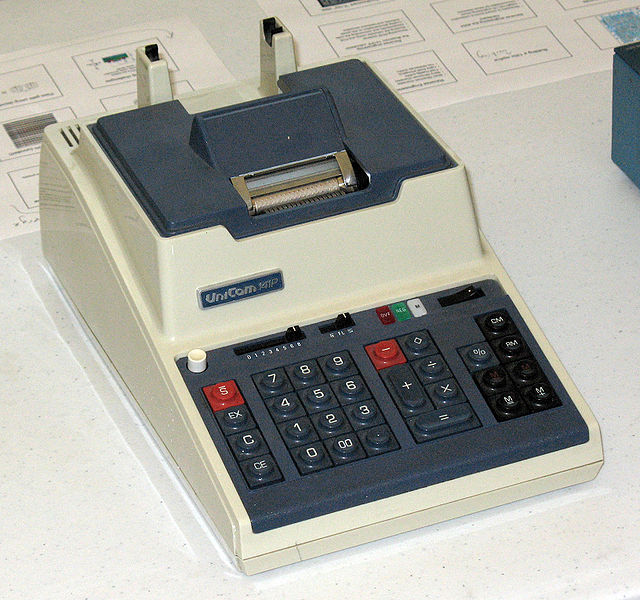
\includegraphics[width=.5\textwidth]{images/i4004-calculator.jpg}\\
    \begin{tiny}
      \emph{Unicom 141P Calculator 3} foto de Michael Holley.\\ 
    \end{tiny}
  \end{column}
\end{columns}
\end{frame}

\begin{frame}[t]{Efectos de los microprocesadores}
\begin{itemize}
  \item \textmark{Producción en masa} de microprocesadores.
    \begin{itemize}
      \item Fuerte reducción de coste unitario.
      \item Crecimiento de la fracción de computadores basados en microprocesadores.
    \end{itemize}

  \mode<presentation>{\vfill\pause}
  \item \textgood{Cambios significativos} en el mercado:
    \begin{itemize}
      \item \textbad{Eliminación} casi total de la necesidad de 
            \textmark{programación en ensamblador}.
      \item \textmark{Sistemas operativos} \textmark{estandarizados} e independientes 
            del fabricante.
        \begin{itemize}
          \item UNIX $\rightarrow$ Linux.
        \end{itemize}
      \item \textgood{Reducción de costes} para nuevas arquitecturas.
    \end{itemize}
\end{itemize}
\end{frame}

\begin{frame}[t]{Segunda revolución}
\begin{itemize}
  \item Extracción del paralelismo implícito a nivel de instrucción (ILP).
    \begin{itemize}
      \item El hardware tiene recursos que pueden usarse en paralelo.
    \end{itemize}
  \mode<presentation>{\vfill}
  \pause
  \item \textgood{Elementos}:
    \begin{itemize}[<+->]
      \item \textmark{Segmentación}: Permitió incrementar frecuencias de reloj.
      \item \textmark{Cachés}: Necesarias para incrementar las frecuencias de reloj.
      \item \textmark{Coma flotante}: Integradas en el chip.
      \item Incremento en la \textmark{profundidad del pipeline} y \textmark{especulación de salto}.
      \item \textmark{Emisión múltiple}: Arquitecturas superescalares.
      \item \textmark{Planificación dinámica}: Ejecución fuera de orden.
    \end{itemize}
\end{itemize}
\end{frame}

\begin{frame}[t,shrink=15]{Culminación de procesadores de un núcleo}
\begin{columns}
  \begin{column}{.15\textwidth}
    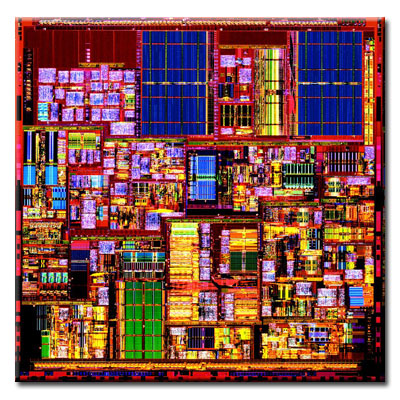
\includegraphics[width=\textwidth]{images/intel-p4-die.jpg}\\
    \begin{tiny}
      Die of Intel Pentium 4 (Northwood)\\
      Source: \url{http://gecko54000.free.fr}\\
    \end{tiny}
    \vspace{0.75em}
    \begin{center}
      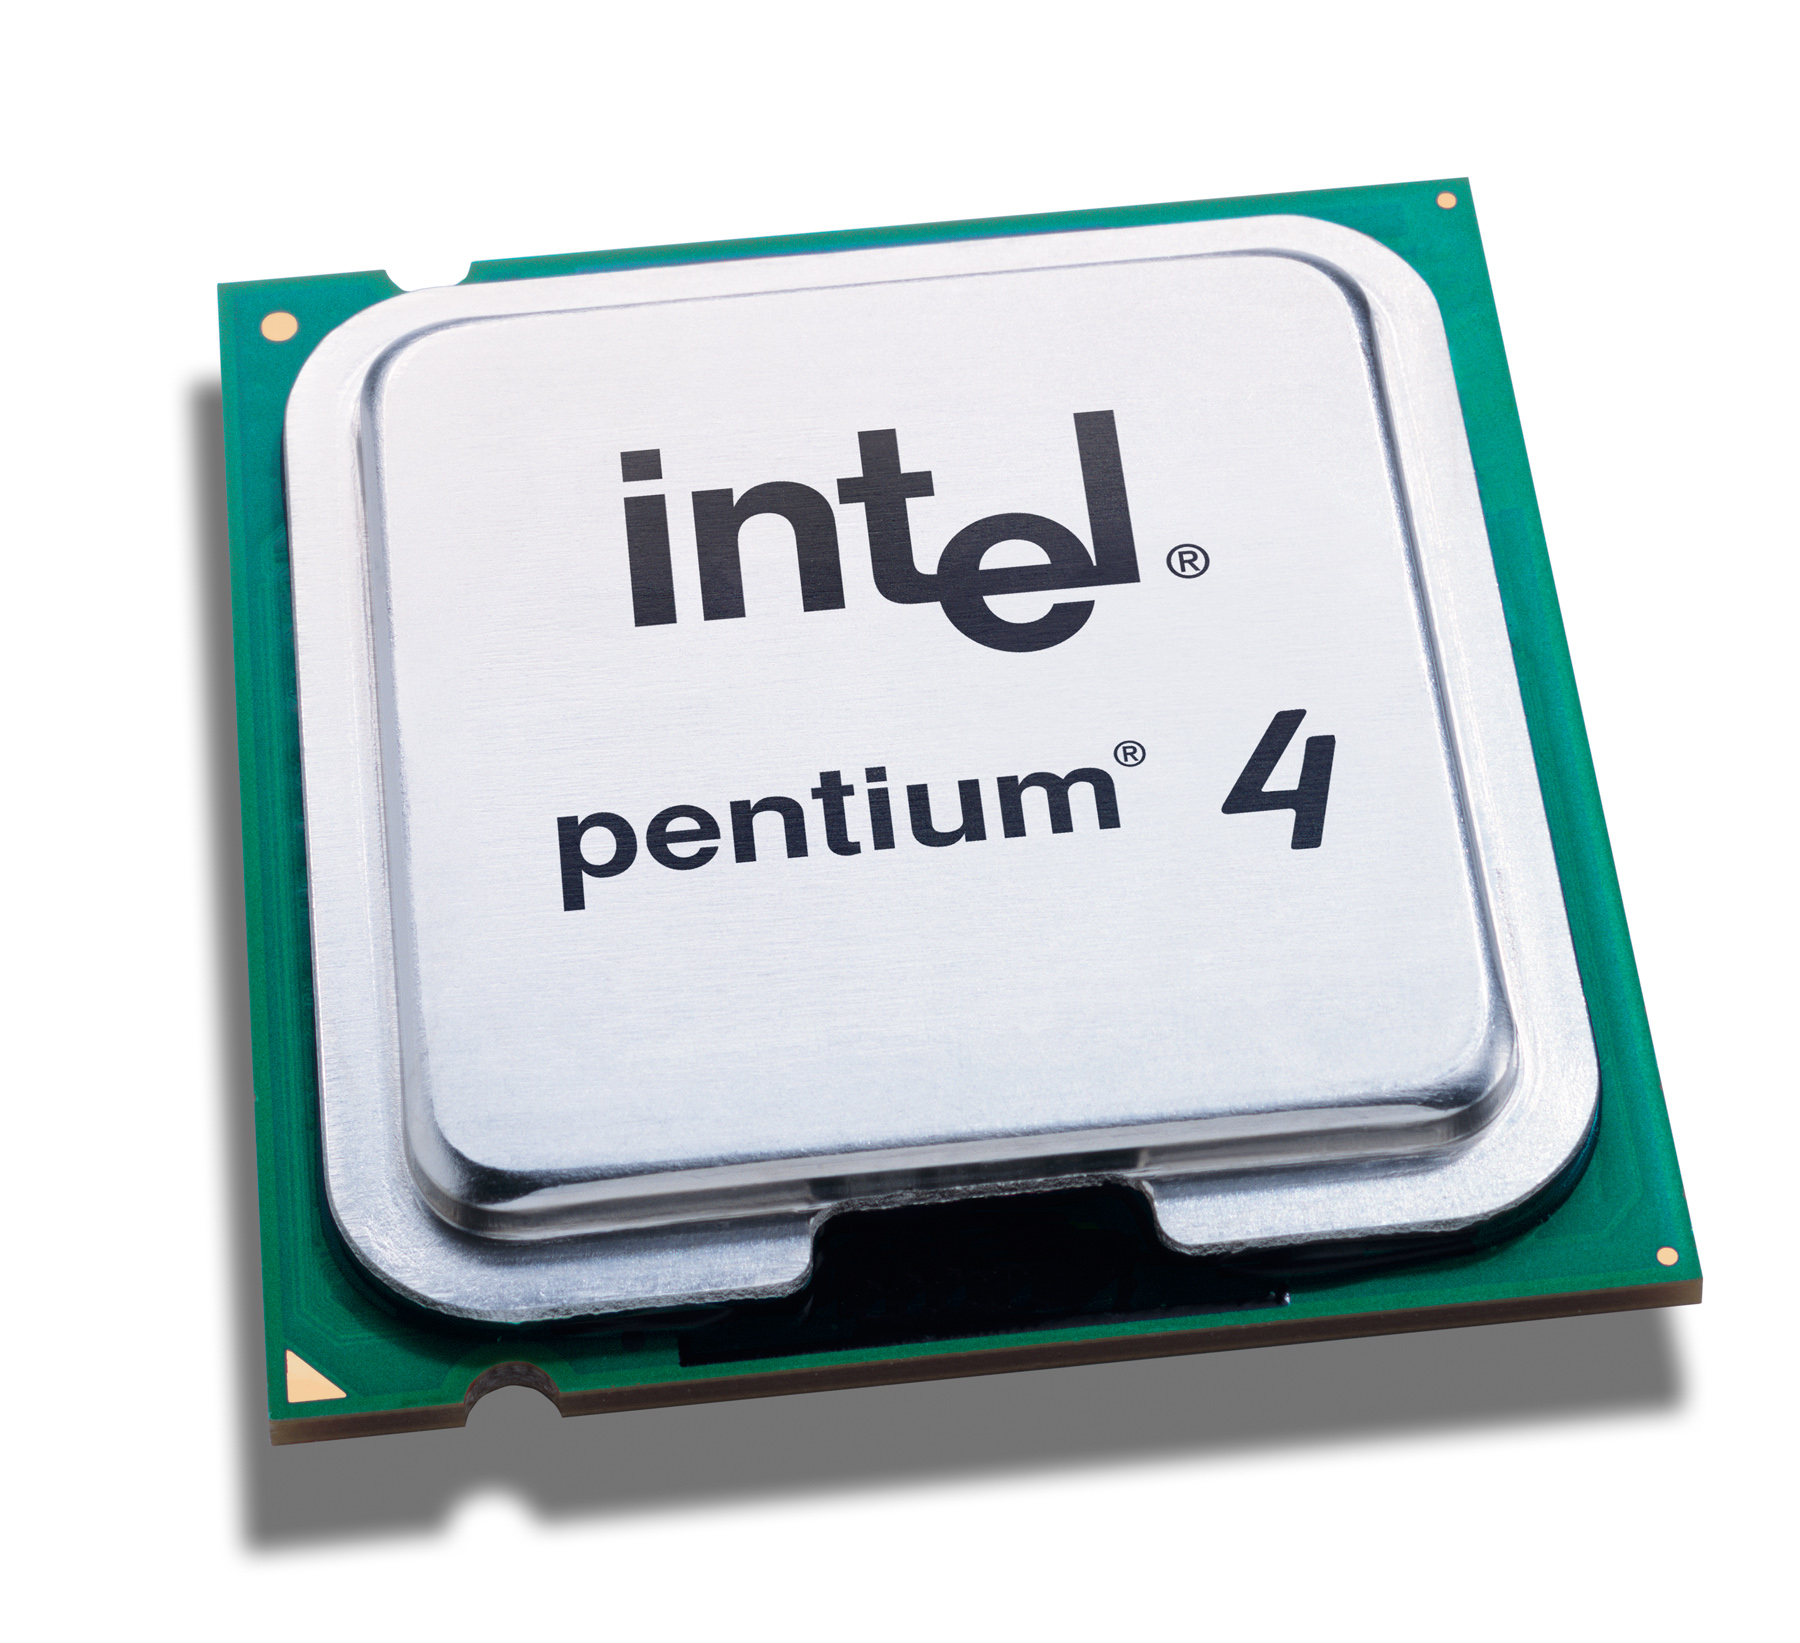
\includegraphics[width=.9\textwidth]{images/intel-p4.jpg}\\
    \end{center}
  \end{column}
  \begin{column}{.7\textwidth}
    \begin{itemize}
      \item Intel Pentium 4 (2003).
        \begin{itemize}
          \item \textmark{Dominio de aplicación}: Escritorio/Servidor.
          \item \textmark{Tecnología}: 90 nm (1/100x).
        \end{itemize}
      \item \textgood{Datos}:
        \begin{itemize}
          \item 55M transistores (20,000x).
          \item 101 mm$^2$ (10x).
          \item 3.4 GHz (10,000x).
          \item 1.2 Volts (1/10x).
        \end{itemize}
      \item \textgood{Características}:
        \begin{itemize}
          \item Datos de 32/64 bits (16x).
          \item Segmentación en 22 etapas (más tarde 31).
          \item 3-4 instrucciones por ciclo (superescalar).
          \item Dos niveles de caché en chip.
          \item Paralelismo de datos (SIMD).
          \item \emph{Hyper-threading}.
        \end{itemize}
    \end{itemize}
  \end{column}
\end{columns}
\end{frame}

\begin{frame}[t]{Tercera revolución}
\begin{itemize}
  \item Soporte a paralelismo explícito de datos y de hilos.
    \begin{itemize}
      \item Hardware ofrece recursos paralelos y software especifica su uso.
      \item El paralelismo deja de ser ocultado por el hardware.
      \item \textmark{Razón}: Beneficios cada vez menores de ILP.
    \end{itemize}
  \mode<presentation>{\vfill}
  \pause
  \item \textgood{Elementos}:
    \begin{itemize}
      \item \textmark{Instrucciones vectoriales}: Intel SSE, AVX, AVX-2, \ldots
      \item Soporte general para aplicaciones \textmark{multi-hilo}.
    \end{itemize}
\end{itemize}
\end{frame}

\begin{frame}[t,shrink=20]{Procesadores multi-core}
\begin{columns}[T]
  \begin{column}{.65\textwidth}
    \begin{itemize}
      \item Intel Core i7 (2009).
        \begin{itemize}
          \item \textmark{Dominio de aplicación}: Escritorio / Servidor.
          \item \textmark{Tecnología}: 45 nm (1/2x).
        \end{itemize}
      \mode<presentation>{\vfill}
      \item \textgood{Datos}:
        \begin{itemize}
          \item 774M transistores (12x).
          \item 296 mm$^2$ (3x).
          \item 3.2 GHz -- 3.6 GHz ($\approx$1x).
          \item 0.7 -- 1.4 Voltios ($\approx$1x).
        \end{itemize}
      \mode<presentation>{\vfill}
      \item \textgood{Características}:
        \begin{itemize}
          \item Datos de 128 bits (2x).
          \item Segmentación de 14 etapas (0.5x).
          \item 4 instrucciones por ciclo ($\approx$1x).
          \item Tres niveles de caché en chip.
          \item SIMD, \emph{hyper-threading}
          \item 4 cores (4x).
        \end{itemize} 
    \end{itemize}
  \end{column}
  \begin{column}{.35\textwidth}
    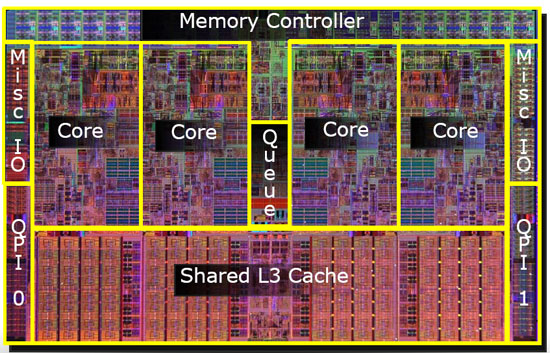
\includegraphics[width=.9\textwidth]{images/intel-core-i7-die.jpg}\\
    \begin{tiny}
      Die of Intel Core i7 (Nehalem)\\
      Source: \url{www.legitreviews.com}\\
    \end{tiny}
    \vfill
    \begin{center}
    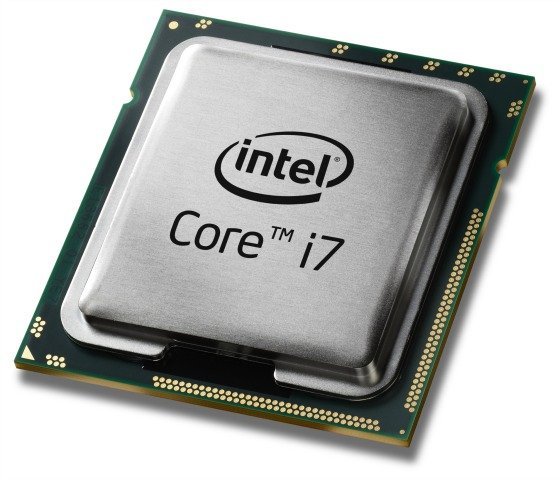
\includegraphics[width=.45\textwidth]{images/intel-core-i7.jpg}\\
    \end{center}
  \end{column}
\end{columns}
\end{frame}

\begin{frame}[t]{Tendencias arquitectónicas}
\begin{itemize}
  \item Paralelismo a nivel de instrucción:
    \begin{itemize}
      \item Ejecución paralela de instrucciones.
      \item Imposible mejorar significativamente ILP desde 2003-2005.
      \item El hardware y el compilador \emph{conspiran} para ocultar detalles al programador.
        \begin{itemize}
          \item Programador con vista \alert{muy simplificada} del hardware.
        \end{itemize}
    \end{itemize}
  \mode<presentation>{\pause\vfill}
  \item Nuevos modelos para mejorar rendimiento:
    \begin{itemize}
       \item \textmark{Data-Level} Parallelism (DLP).
       \item \textmark{Thread-Level} Parallelism (TLP).
       \item \textmark{Request-Level} Parallelism (RLP).
    \end{itemize}
  \mode<presentation>{\pause\vfill}
  \item \alert{IMPORTANTE}: Todos ellos requieren reestructurar las aplicaciones
        para conseguir los incrementos de rendimiento prometidos.
\end{itemize}
\end{frame}
